\documentclass[11pt,a4paper]{article}
\usepackage[utf8]{inputenc}
\usepackage{amsmath}
\usepackage{amsfonts}
\usepackage{amssymb}
\usepackage{graphicx}
\usepackage{multirow}
\usepackage{tikz}
\usetikzlibrary{shapes}
\author{Daniel Deutsch}
\begin{document}

	\begin{center}
	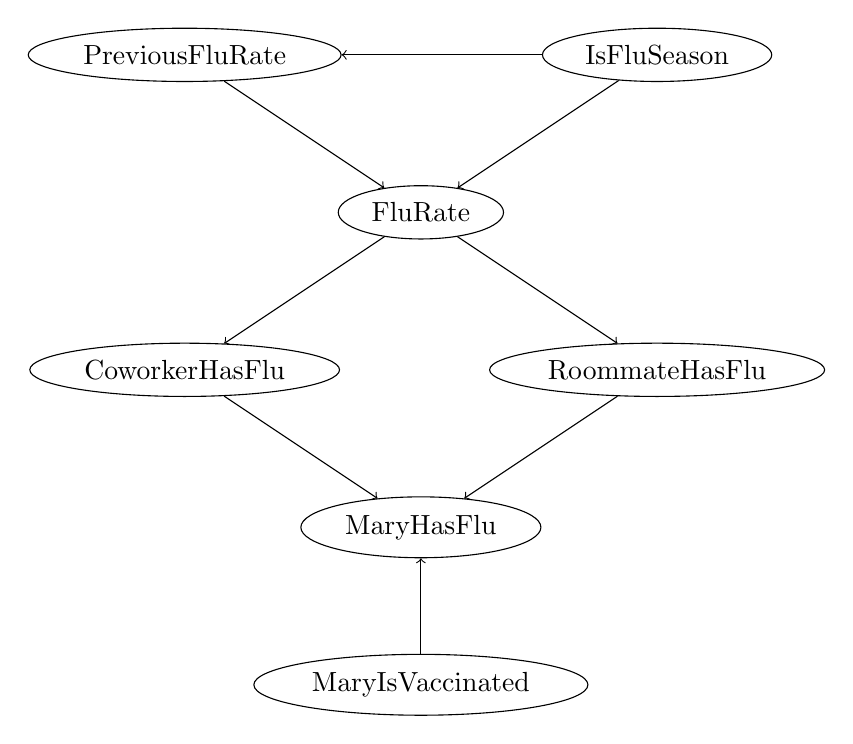
\begin{tikzpicture}

		\node (PreviousFluRate) at (0,8) [draw,shape=ellipse]{PreviousFluRate};		
		\node (IsFluSeason) at (6,8) [draw,shape=ellipse]{IsFluSeason};		

		\node (FluRate) at (3,6) [draw,shape=ellipse]{FluRate};		
		
		\node (CoworkerHasFlu) at (0,4) [draw,shape=ellipse]{CoworkerHasFlu};		
		\node (RoommateHasFlu) at (6,4) [draw,shape=ellipse]{RoommateHasFlu};				
		
		\node (MaryHasFlu) at (3,2) [draw,shape=ellipse]{MaryHasFlu};				
		
		\node (MaryIsVaccinated) at (3,0) [draw,shape=ellipse]{MaryIsVaccinated};						
		
		\draw [->] (IsFluSeason) -- (PreviousFluRate);
		\draw [->] (IsFluSeason) -- (FluRate);
				
		\draw [->] (PreviousFluRate) -- (FluRate);
		
		\draw [->] (FluRate) -- (CoworkerHasFlu);
		\draw [->] (FluRate) -- (RoommateHasFlu);
		
		\draw [->] (CoworkerHasFlu) -- (MaryHasFlu);
		
		\draw [->] (RoommateHasFlu) -- (MaryHasFlu);
		
		\draw [->] (MaryIsVaccinated) -- (MaryHasFlu);
	\end{tikzpicture}
	\end{center}
	
	
% PREVIOUS FLU RATE	
\begin{tabular}{|c|c|c|c|}
\hline 
 & \multicolumn{3}{|c|}{\textbf{PreviousFluRate}}  \\ 
\hline 
\textbf{IsFluSeason} & Mild & Moderate & Severe \\ 
\hline 
0 & 0.85 & 0.1 & 0.05 \\ 
\hline 
1 & 0.15 & 0.55 & 0.3 \\ 
\hline 
\end{tabular} 

% FLU RATE
\begin{tabular}{|c|c|c|c|c|}
\hline 
\multicolumn{2}{|c|}{} & \multicolumn{3}{|c|}{\textbf{FluRate}} \\ 
\hline 
\textbf{PreviousFluRate} & \textbf{IsFluSeason} & Mild & Moderate & Severe \\ 
\hline 
Mild & 0 & 0.9 & 0.08 & 0.02 \\ 
\hline 
Mild & 1 & 0.3 & 0.5 & 0.2 \\ 
\hline 
Moderate & 0 & 0.85 & 0.1 & 0.05 \\ 
\hline 
Moderate & 1 & 0.1 & 0.65 & 0.25 \\ 
\hline 
Severe & 0 & 0.7 & 0.2 & 0.1 \\ 
\hline 
Severe & 1 & 0.05 & 0.1 & 0.75 \\ 
\hline 
\end{tabular} 

% COWORKER HAS FLU
\begin{tabular}{|c|c|c|}
\hline 
 & \multicolumn{2}{|c|}{\textbf{CoworkerHasFlu}} \\ 
\hline 
\textbf{FluRate} & 0 & 1 \\ 
\hline 
Mild & 0.8 & 0.2 \\ 
\hline 
Moderate & 0.5 & 0.5 \\ 
\hline 
Severe & 0.2 & 0.8 \\ 
\hline 
\end{tabular} 

% ROOMATE HAS FLU
\begin{tabular}{|c|c|c|}
\hline 
 & \multicolumn{2}{|c|}{\textbf{RoommateHasFlu}} \\ 
\hline 
\textbf{FluRate} & 0 & 1 \\ 
\hline 
Mild & 0.8 & 0.2 \\ 
\hline 
Moderate & 0.5 & 0.5 \\ 
\hline 
Severe & 0.2 & 0.8 \\ 
\hline 
\end{tabular} 

\begin{tabular}{|c|c|c|c|c|}
\hline 
\multicolumn{3}{|c|}{} & \multicolumn{2}{|c|}{\textbf{MaryHasFlu}}  \\ 
\hline 
\textbf{MaryIsVaccinated} & \textbf{RoomateHasFlu} & \textbf{CoworkerHasFlu} & 0 & 1 \\ 
\hline 
0 & 0 & 0 & 0.9 & 0.1 \\ 
\hline 
0 & 0 & 1 & 0.6 & 0.4 \\ 
\hline 
0 & 1 & 0 & 0.45 & 0.55 \\ 
\hline 
0 & 1 & 1 & 0.2 & 0.8 \\ 
\hline 
1 & 0 & 0 & 0.99 & 0.01 \\ 
\hline 
1 & 0 & 1 & 0.95 & 0.05 \\ 
\hline 
1 & 1 & 0 & 0.9 & 0.1 \\ 
\hline 
1 & 1 & 1 & 0.85 & 0.15 \\ 
\hline 
\end{tabular} 

\end{document}